\begin{landscape}
\subsection{Approximation des Bode-Diagramms}
\renewcommand{\arraystretch}{1.5}
\begin{longtable}{|l|l|ll|ll|}
	\hline
		\textbf{Pole} & 
		\textbf{UTF} $H(s)$ &
		\multicolumn{2}{c}{\textbf{Amplitude} $|H(s)|$} & 
		\multicolumn{2}{|c|}{\textbf{Phase} $\angle(H(s))$}
	\\ \hline
		Keine, konstanter Faktor &
		$\alpha e^{j \beta}$ &
		\parbox[c][1cm]{1cm}{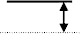
\includegraphics[width=1cm]{./images/bode-approx-konst.png}} &
		\, Konstant: $20 \log \alpha$ &
		\parbox[c][1cm]{1cm}{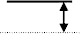
\includegraphics[width=1cm]{./images/bode-approx-konst.png}} &
		Konstant: $\beta$
	\\ \hline
		Pol im Ursprung &
		$\frac{\alpha}{s}$ &
		\parbox[c][1cm]{1cm}{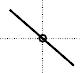
\includegraphics[width=1cm]{./images/bode-approx-ampl-tp-ord1.png}} & 
		\begin{tabular}{l}
			Lineare Steigung: $-20 dB/Dek.$ \\
			$0dB$ bei $\omega = \alpha$
		\end{tabular} &
		\parbox[c][1cm]{1cm}{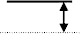
\includegraphics[width=1cm]{./images/bode-approx-konst.png}} & 
		Konstant: $-\frac{\pi}{2}$ 
	\\ \hline
		Nullstelle im Ursprung &
		$\alpha s$ &
		\parbox[c][1cm]{1cm}{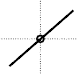
\includegraphics[width=1cm]{./images/bode-approx-ampl-hp-ord1.png}} & 
		\begin{tabular}{l}
			Lineare Steigung: $+20 dB/Dek.$ \\
			$0dB$ bei $\omega = \frac{1}{\alpha}$
		\end{tabular} &
		\parbox[c][1cm]{1cm}{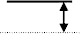
\includegraphics[width=1cm]{./images/bode-approx-konst.png}} &
		Konstant: $+\frac{\pi}{2}$
	\\ \hline	
		Reeller Pol &
		$\frac{1}{s + \alpha}$ &
		\parbox[c][1cm]{1cm}{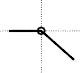
\includegraphics[width=1cm]{./images/bode-approx-ampl-4.png}} &
		\begin{tabular}{ll}
			$\omega < \alpha$: & Konstant $-20 \log \alpha$  \\
			$\omega > \alpha$: & $-20dB/Dek.$
		\end{tabular} &
		\parbox[c][1cm]{1cm}{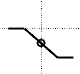
\includegraphics[width=1cm]{./images/bode-approx-phase-4.png}} &
		\begin{tabular}{ll}
			$\omega < \frac{\alpha}{10} $:	& Konstant $0$ \\
			$\omega > 10 \alpha$:		& Konstant $-\frac{\pi}{2}$
		\end{tabular}
	\\ \hline
		Reeller Pol &
		$\frac{\alpha}{s + \alpha}$ &
		\parbox[c][1cm]{1cm}{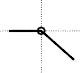
\includegraphics[width=1cm]{./images/bode-approx-ampl-4.png}} &
		\begin{tabular}{ll}
			$\omega < \alpha$: & Konstant $0dB$ \\
			$\omega > \alpha$: & $-20dB/Dek.$
		\end{tabular} &
		\parbox[c][1cm]{1cm}{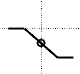
\includegraphics[width=1cm]{./images/bode-approx-phase-4.png}}	& 
		\begin{tabular}{ll}
			$\omega < \frac{\alpha}{10}$: & Konstant $0$ \\
			$\omega > 10 \alpha$: & Konstant $-\frac{\pi}{2}$
		\end{tabular}
	\\ \hline
		Reelle Nullstelle &
		$s + \alpha$ & 
		\parbox[c][1cm]{1cm}{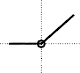
\includegraphics[width=1cm]{./images/bode-approx-ampl-5.png}} &
		\begin{tabular}{ll}
			$\omega < \alpha$: & Konstant $20 \log \alpha$ \\
			$\omega > \alpha$: & $+20dB/Dek.$
		\end{tabular} & 
		\parbox[c][1cm]{1cm}{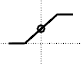
\includegraphics[width=1cm]{./images/bode-approx-phase-5.png}}	&
		\begin{tabular}{ll}
			$\omega < \frac{\alpha}{10}$: & Konstant $0$ \\
			$\omega > 10 \alpha$: & Konstant $+\frac{\pi}{2}$
		\end{tabular}
	\\ \hline	
		Reelle Nullstelle &
		$\frac{s + \alpha}{\alpha}$ &
		\parbox[c][1cm]{1cm}{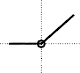
\includegraphics[width=1cm]{./images/bode-approx-ampl-5.png}} &
		\begin{tabular}{ll}
			$\omega < \alpha$: & Konstant $0dB$ \\
			$\omega > \alpha$: & $+20dB/Dek.$
		\end{tabular} &
		\parbox[c][1cm]{1cm}{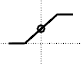
\includegraphics[width=1cm]{./images/bode-approx-phase-5.png}} &
		\begin{tabular}{ll}
			$\omega < \frac{\alpha}{10}$: & Konstant $0$ \\
			$\omega > 10 \alpha$: & Konstant $+\frac{\pi}{2}$
		\end{tabular}
	\\ \hline
		Konjugiert-komplexe Pole &
		$\frac{1}{s^2+s\frac{\omega_p}{q_p}+\omega_p^2}$ &
		\parbox[c][1cm]{1cm}{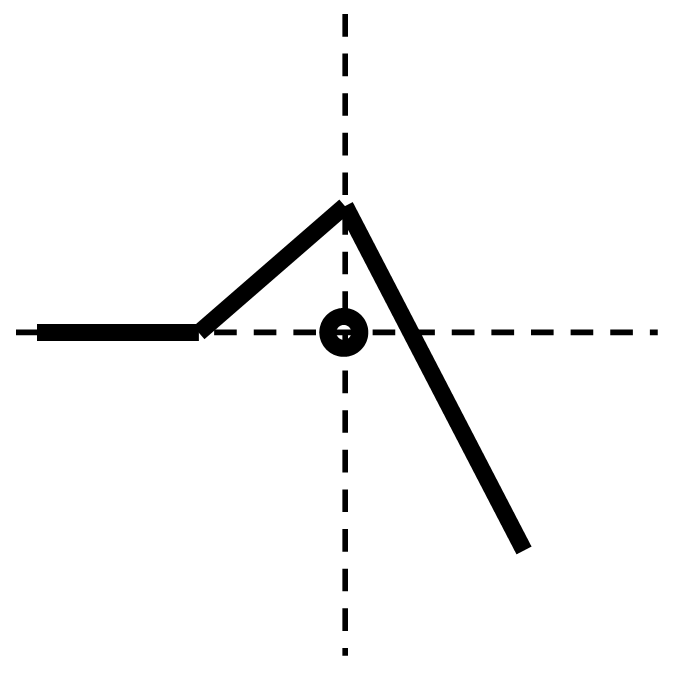
\includegraphics[width=1cm]{./images/bode-approx-ampl-6.png}} &
		\begin{tabular}{ll}
			$\omega < \omega_p$: 	& Konstant $-40 \log \omega_p$ \\
			$\omega > \omega_p$:	& $-40dB/Dek.$ \\
			Überhöhung: 			& $\frac{\omega_p}{2}$ bis $2\omega_p$ \\
			Maximum:				& $20 \log q_p$ bei $\omega = \omega_p$			
		\end{tabular} &
		\parbox[c][1cm]{1cm}{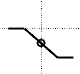
\includegraphics[width=1cm]{./images/bode-approx-phase-6.png}} &
		\begin{tabular}{ll}
			$\omega < \frac{\omega_p}{10^{\frac{1}{2q_p}}}$:	& Konstant $0$ \\
			$\omega > \omega_p 10^{\frac{1}{2q_p}}$:			& Konstant $-\pi$ \\
			$\omega = \omega_p$:								& $-\frac{\pi}{2}$
		\end{tabular}
	\\ \hline
		Konjugiert-komplexe Pole &
		$\frac{\omega_p^2}{s^2+s\frac{\omega_p}{q_p}+\omega_p^2}$ & 
		\parbox[c][1cm]{1cm}{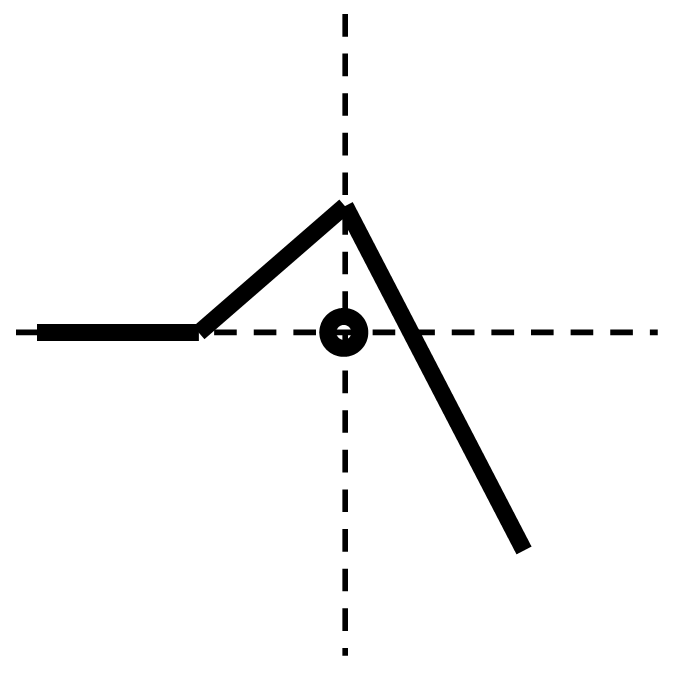
\includegraphics[width=1cm]{./images/bode-approx-ampl-6.png}} &
		\begin{tabular}{ll}
			$\omega < \omega_p$:	& Konstant $0dB$ \\
			$\omega > \omega_p$:	& $-40dB/Dek.$ \\
			Überhöhung:				& $\frac{\omega_p}{2}$ bis $2 \omega_p$ \\
			Maximum:				& $20 \log q_p$ bei $\omega = \omega_p$
		\end{tabular} &
		\parbox[c][1cm]{1cm}{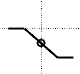
\includegraphics[width=1cm]{./images/bode-approx-phase-6.png}}	& 
		\begin{tabular}{ll}
			$\omega < \frac{\omega_p}{10^{\frac{1}{2q_p}}}$:	& Konstant $0$ \\
			$\omega > \omega_p 10^{\frac{1}{2q_p}}$:			& Konstant $-\pi$ \\
			$\omega = \omega_p$:								& $-\frac{\pi}{2}$
		\end{tabular}
	\\ \hline	
		Konjugiert-komplexe Nullstellen &
		$s^2+s\frac{\omega_z}{q_z}+\omega_z^2$ &
		\multicolumn{4}{l|}{
			Analog zu den Konjugiert-komplexen Polen jedoch gespiegelt an der $0dB$- / $0$-Grad-Linie.
		}
	\\
		&
		$\frac{s^2+s\frac{\omega_z}{q_z}+\omega_z^2}{\omega_z^2}$ &
		\multicolumn{4}{l|}{}
	\\ \hline
		\multicolumn{6}{|p{21cm}|}{
			Serieschaltung von Systemen erfolgt durch \textbf{Superposition} der einzelnen Bode-Diagramme 
			(Multiplikation von UTFs entspricht Addition im	dB-Bereich).
		}
	\\ \hline
\end{longtable}
\renewcommand{\arraystretch}{\arraystretchOriginal}
\end{landscape}